\documentclass[11pt,a4paper]{article}

\usepackage[english]{babel}
\usepackage{geometry}
\geometry{margin=2.2cm}
\usepackage{graphicx}
\usepackage{xcolor}
\usepackage{booktabs}
\usepackage{array}
\usepackage{listings}
\usepackage{caption}
\usepackage{titlesec}
\usepackage{fancyhdr}
\usepackage{hyperref}
\usepackage{enumitem}

\definecolor{codebg}{RGB}{245,246,248}
\definecolor{codeframe}{RGB}{205,210,218}
\definecolor{linkblue}{RGB}{16,78,139}
\definecolor{okgreen}{RGB}{22,120,60}
\definecolor{failred}{RGB}{170,30,30}

\hypersetup{colorlinks=true, linkcolor=linkblue, urlcolor=linkblue, citecolor=linkblue}

\lstdefinestyle{shell}{
  backgroundcolor=\color{codebg},
  frame=single,
  rulecolor=\color{codeframe},
  basicstyle=\ttfamily\scriptsize,
  breaklines=true,
  breakatwhitespace=false,
  columns=fullflexible,
  keepspaces=true,
  showstringspaces=false,
  captionpos=b
}
\lstset{style=shell}

\titleformat{\section}{\large\bfseries\color{linkblue}}{\thesection.}{0.6em}{}
\titleformat{\subsection}{\normalsize\bfseries}{\thesubsection}{0.5em}{}

\pagestyle{fancy}
\fancyhf{}
\fancyhead[L]{\footnotesize DevOps \& Cloud Computing --- Lab No. 07}
\fancyhead[R]{\footnotesize Sadoune Fadjr --- Group 02 --- ING 5}
\fancyfoot[C]{\footnotesize\thepage}
\renewcommand{\headrulewidth}{0.4pt}

\begin{document}

\begin{titlepage}
\centering
\vspace*{1.2cm}
{\large Department of Computer Science}\\[0.3cm]
{\large 5\textsuperscript{th} year --- Software Engineering (ING 5)}\\[2.0cm]

{\Huge\bfseries Lab Report No. 07}\\[0.6cm]
{\LARGE Building a CI/CD Pipeline\\[0.2cm] with Jenkins and Docker}\\[2.2cm]

\rule{\linewidth}{0.4pt}\\[0.6cm]
{\large\bfseries Submitted by}\\[0.3cm]
{\Large Sadoune Fadjr}\\[0.3cm]
{\large Group 02 --- ING 5}\\[0.6cm]
\rule{\linewidth}{0.4pt}\\[2.0cm]

{\large Module: DevOps \& Cloud Computing}\\[3.0cm]

{\large Academic year 2026--2027}\\[0.3cm]
{\large \today}
\vfill
\end{titlepage}

\tableofcontents
\newpage

\section{Introduction and objectives}

This report presents Lab No. 07: building a Continuous Integration and Continuous
Delivery (CI/CD) pipeline with \textbf{Jenkins} and \textbf{Docker} around a small
\textbf{Flask} application.

The objectives of the lab are to:
\begin{itemize}[leftmargin=1.2cm]
  \item explain the role of Jenkins in Continuous Integration and Continuous Delivery;
  \item understand the main components of a Jenkins pipeline;
  \item connect a Jenkins job to a GitHub repository;
  \item build a Docker image automatically;
  \item run automated tests as part of the pipeline;
  \item deploy the application and verify that it is available;
  \item show that a failed test prevents an unsuccessful version from being deployed.
\end{itemize}

The work was carried out on a \textbf{Windows} machine with \textbf{Docker Desktop}
(Linux containers), Jenkins itself running inside a Docker container.
Two adaptations were required compared with the instructions written for a Linux host:
\begin{enumerate}[leftmargin=1.2cm]
  \item the official Jenkins image does not include the Docker client, so a derived image
        containing the \texttt{docker} binary was built and the Docker socket was mounted
        into the Jenkins container;
  \item the \texttt{curl} verification steps use the application container name (shared
        Docker network) and \texttt{host.docker.internal} instead of \texttt{localhost},
        because \texttt{localhost} inside the Jenkins container refers to Jenkins itself.
\end{enumerate}

\section{Architecture and environment}

\subsection{Workflow architecture}

The workflow of the lab is:
\begin{center}
\textbf{GitHub} $\rightarrow$ \textbf{Jenkins Pipeline} $\rightarrow$
\textbf{Docker Image} $\rightarrow$ \textbf{Docker Container} $\rightarrow$
\textbf{Flask Application}
\end{center}

The application is exposed on \texttt{http://localhost:8081} and Jenkins on
\texttt{http://localhost:8080}.

\subsection{Technical environment}

\begin{table}[h!]
\centering
\caption{Versions used on the workstation}
\begin{tabular}{@{}ll@{}}
\toprule
Component & Version / configuration \\
\midrule
Operating system & Windows, Docker Desktop 4.50.0 (Linux containers) \\
Docker engine & 28.5.1 \\
Docker client (inside Jenkins) & 28.5.1 (static binary) \\
Jenkins & 2.541.3 (image \texttt{jenkins/jenkins:lts-jdk17}) \\
Custom Jenkins image & \texttt{jenkins-docker-lab} \\
Git & 2.47.3 \\
Application Python & 3.12 (\texttt{python:3.12-slim}) \\
pytest & 9.2.0 \\
\bottomrule
\end{tabular}
\end{table}

\subsection{Containerizing Jenkins}

The \texttt{jenkins-docker-lab} image is built from
\texttt{jenkins/jenkins:lts-jdk17} and adds the Docker client and \texttt{curl}:

\begin{lstlisting}[caption={Dockerfile of the Jenkins image (outside the application repository).}]
FROM jenkins/jenkins:lts-jdk17
USER root
RUN apt-get update \
    && apt-get install -y --no-install-recommends ca-certificates curl \
    && rm -rf /var/lib/apt/lists/* \
    && curl -fsSL https://download.docker.com/linux/static/stable/x86_64/docker-28.5.1.tgz \
       | tar xz -C /tmp \
    && mv /tmp/docker/docker /usr/local/bin/docker \
    && rm -rf /tmp/docker
USER jenkins
\end{lstlisting}

The Jenkins container is started with the Docker socket mounted and on a dedicated
network shared with the application container:

\begin{lstlisting}
docker network create jenkins-net
docker run -d --name jenkins --network jenkins-net -u root \
  -p 8080:8080 -p 50000:50000 \
  -v //var/run/docker.sock:/var/run/docker.sock \
  -v jenkins_home:/var/jenkins_home jenkins-docker-lab
\end{lstlisting}

\section{Project structure and GitHub repository}

\subsection{Repository structure}

\begin{lstlisting}
jenkins-flask-lab/
|-- app.py
|-- requirements.txt
|-- Dockerfile
|-- Jenkinsfile
|-- tests/
|   `-- test_app.py
`-- (extra files: .gitignore, .gitattributes, RAPPORT_Lab07.md)
\end{lstlisting}

The public repository is available at:
\url{https://github.com/Sadoune321/jenkins-flask-lab}

\subsection{Flask application}

\begin{lstlisting}[caption={app.py}]
import os
from flask import Flask, jsonify

app = Flask(__name__)

@app.route("/")
def home():
    version = os.getenv("APP_VERSION", "local")
    return f"<h1>Jenkins CI/CD Lab</h1><p>Version: {version}</p>"

@app.route("/health")
def health():
    return jsonify(status="ok"), 200

if __name__ == "__main__":
    app.run(host="0.0.0.0", port=8000)
\end{lstlisting}

\subsection{Dependencies and Dockerfile}

\begin{lstlisting}[caption={requirements.txt}]
Flask
pytest
gunicorn
\end{lstlisting}

\begin{lstlisting}[caption={Dockerfile of the application.}]
FROM python:3.12-slim
WORKDIR /app
COPY requirements.txt .
RUN pip install --no-cache-dir -r requirements.txt
COPY app.py .
COPY tests ./tests
ENV PYTHONPATH=/app
EXPOSE 8000
CMD ["gunicorn", "--bind", "0.0.0.0:8000", "app:app"]
\end{lstlisting}

The line \texttt{ENV PYTHONPATH=/app} was added after an initial pipeline failure: pytest
could not find the \texttt{app} module during the import
(\texttt{ModuleNotFoundError: No module named 'app'}), because the working directory was
not on the Python path when the tests ran inside the container.

\subsection{Automated tests}

\begin{lstlisting}[caption={tests/test\_app.py}]
from app import app

def test_home():
    response = app.test_client().get("/")
    assert response.status_code == 200
    assert b"Jenkins CI/CD Lab" in response.data

def test_health():
    response = app.test_client().get("/health")
    assert response.status_code == 200
    assert response.get_json() == {"status": "ok"}
\end{lstlisting}

\section{The Jenkins pipeline}

\subsection{The Jenkinsfile}

The declarative pipeline has five stages: Checkout, Build, Test, Deploy and Verify.

\begin{lstlisting}[caption={Jenkinsfile (Linux version used by Jenkins).}]
pipeline {
    agent any
    environment {
        IMAGE_NAME     = 'jenkins-flask-lab'
        CONTAINER_NAME = 'jenkins-flask-app'
        APP_PORT       = '8081'
        NETWORK_NAME   = 'jenkins-net'
    }
    stages {
        stage('Checkout') {
            steps { echo 'Source code is available in the workspace.' }
        }
        stage('Build') {
            steps { sh 'docker build -t ${IMAGE_NAME}:${BUILD_NUMBER} .' }
        }
        stage('Test') {
            steps { sh 'docker run --rm ${IMAGE_NAME}:${BUILD_NUMBER} pytest -v' }
        }
        stage('Deploy') {
            steps {
                sh '''
                    docker rm -f ${CONTAINER_NAME} || true
                    docker run -d --network ${NETWORK_NAME} --name ${CONTAINER_NAME} \
                        -p ${APP_PORT}:8000 -e APP_VERSION=${BUILD_NUMBER} \
                        ${IMAGE_NAME}:${BUILD_NUMBER}
                '''
            }
        }
        stage('Verify') {
            steps {
                sh 'curl --fail --retry 10 --retry-delay 2 http://${CONTAINER_NAME}:8000/health'
                sh 'curl --fail http://${CONTAINER_NAME}:8000/'
                sh 'curl --fail http://host.docker.internal:${APP_PORT}/health'
            }
        }
    }
    post {
        success { echo 'Pipeline completed successfully.' }
        failure { echo 'Pipeline failed. Check the stage that reported an error.' }
    }
}
\end{lstlisting}

\subsection{Description of the stages}

\begin{table}[h!]
\centering
\caption{Role of each pipeline stage}
\begin{tabular}{@{}p{1.9cm}p{6.5cm}p{5.4cm}@{}}
\toprule
Stage & What Jenkins does & Expected result \\
\midrule
Checkout & Retrieves the repository configured in the job (``Pipeline script from SCM'') & Code and Jenkinsfile available in the workspace \\
Build & \texttt{docker build -t jenkins-flask-lab:\${BUILD\_NUMBER} .} & Image tagged with the build number \\
Test & \texttt{docker run --rm ... pytest -v} & 2 tests pass, otherwise the pipeline stops \\
Deploy & Removes the previous container, then starts the new one & New version running on port 8081 \\
Verify & HTTP requests on \texttt{/health} and \texttt{/} with retries & The application responds successfully \\
\bottomrule
\end{tabular}
\end{table}

\subsection{Job configuration in Jenkins}

The job was created with the name \texttt{jenkins-flask-lab}, of type \textbf{Pipeline},
then configured as \emph{Pipeline script from SCM} with:
\begin{itemize}[leftmargin=1.2cm]
  \item SCM: Git;
  \item Repository URL: \url{https://github.com/Sadoune321/jenkins-flask-lab.git} (public repository, no credentials);
  \item Branch Specifier: \texttt{*/main};
  \item Script Path: \texttt{Jenkinsfile}.
\end{itemize}

\begin{figure}[h!]
\centering
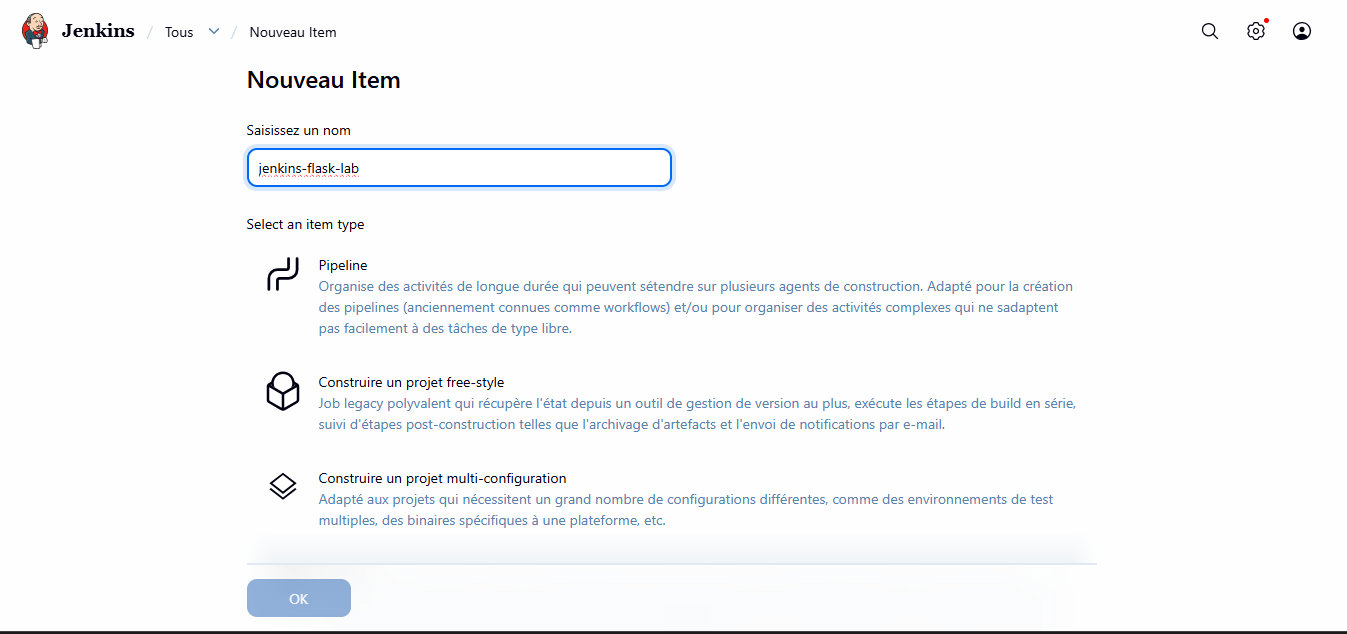
\includegraphics[width=0.92\textwidth]{img/jenkins_new_item.png}
\caption{Creating the Pipeline job \texttt{jenkins-flask-lab} in Jenkins.}
\end{figure}

\section{Results: successful pipeline}

The pipeline runs successfully: the five stages are green, the image is built and tagged
with the build number, both tests pass, the container is deployed and the HTTP checks
succeed.

\begin{figure}[h!]
\centering
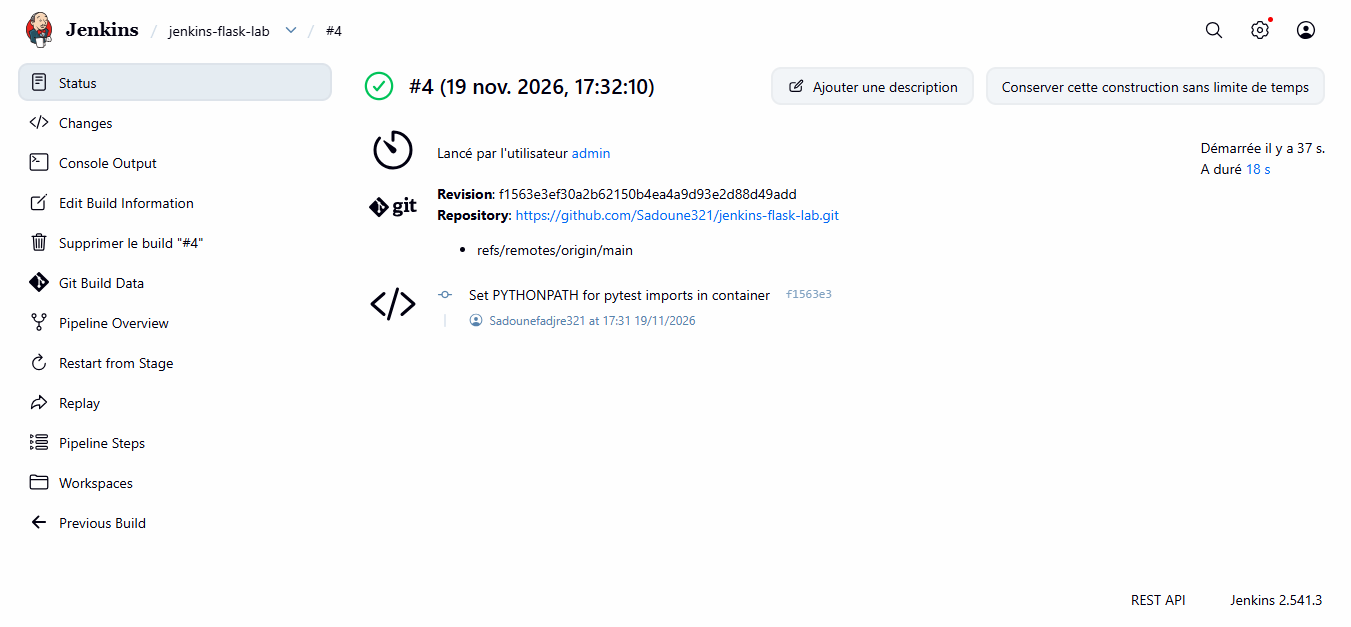
\includegraphics[width=0.92\textwidth]{img/build_success.png}
\caption{Successful build: the pipeline finishes with the SUCCESS status.}
\end{figure}

\begin{figure}[h!]
\centering

\includegraphics[width=0.92\textwidth]{img/app_home.png}
\caption{Deployed application available at \texttt{http://localhost:8081}: the build number is displayed.}
\end{figure}

\begin{figure}[h!]
\centering
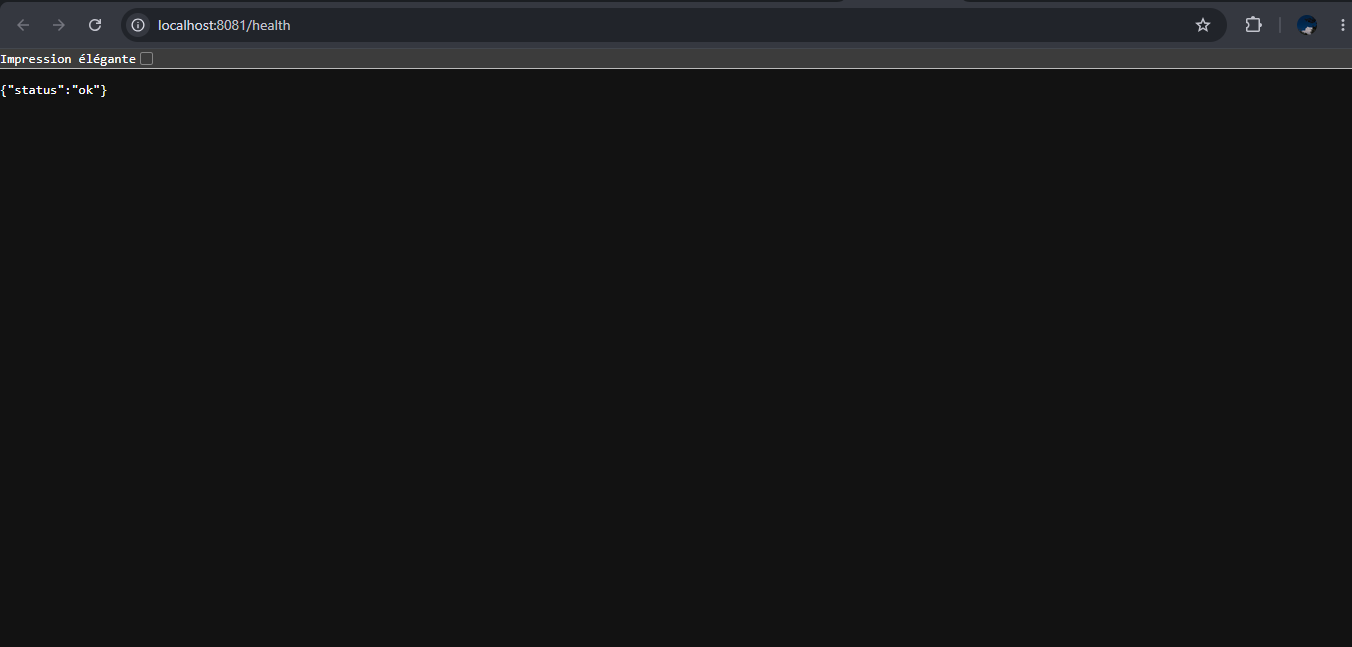
\includegraphics[width=0.92\textwidth]{img/app_health.png}
\caption{Health endpoint \texttt{/health}: response \texttt{\{"status":"ok"\}}.}
\end{figure}

Console output excerpt of a successful build (build 7):

\begin{lstlisting}
Checking out Revision fe1a2252a304087108c619a3a52ce393e8987edf (refs/remotes/origin/main)
+ docker build -t jenkins-flask-lab:7 .
Successfully tagged jenkins-flask-lab:7
tests/test_app.py::test_home PASSED                                      [ 50%]
tests/test_app.py::test_health PASSED                                    [100%]
+ curl --fail --retry 10 --retry-delay 2 http://jenkins-flask-app:8000/health
{"status":"ok"}
+ curl --fail http://jenkins-flask-app:8000/
<h1>Jenkins CI/CD Lab</h1><p>Version: 7</p>
+ curl --fail http://host.docker.internal:8081/health
{"status":"ok"}
Pipeline completed successfully.
Finished: SUCCESS
\end{lstlisting}

\section{Part E: observing a failed pipeline}

To demonstrate that tests protect production, the health test assertion was temporarily
changed:

\begin{lstlisting}
assert response.get_json() == {"status": "incorrect"}
\end{lstlisting}

After committing and pushing (commit \texttt{dd81f24}, message
``Introduce a test failure''), a new build (build 8) was started. As expected:
\begin{itemize}[leftmargin=1.2cm]
  \item the \textbf{Test} stage fails;
  \item the \textbf{Deploy} and \textbf{Verify} stages are skipped;
  \item the build finishes as \textcolor{failred}{\textbf{FAILURE}};
  \item the container of the previous version stays up and is not replaced.
\end{itemize}

\begin{figure}[h!]
\centering
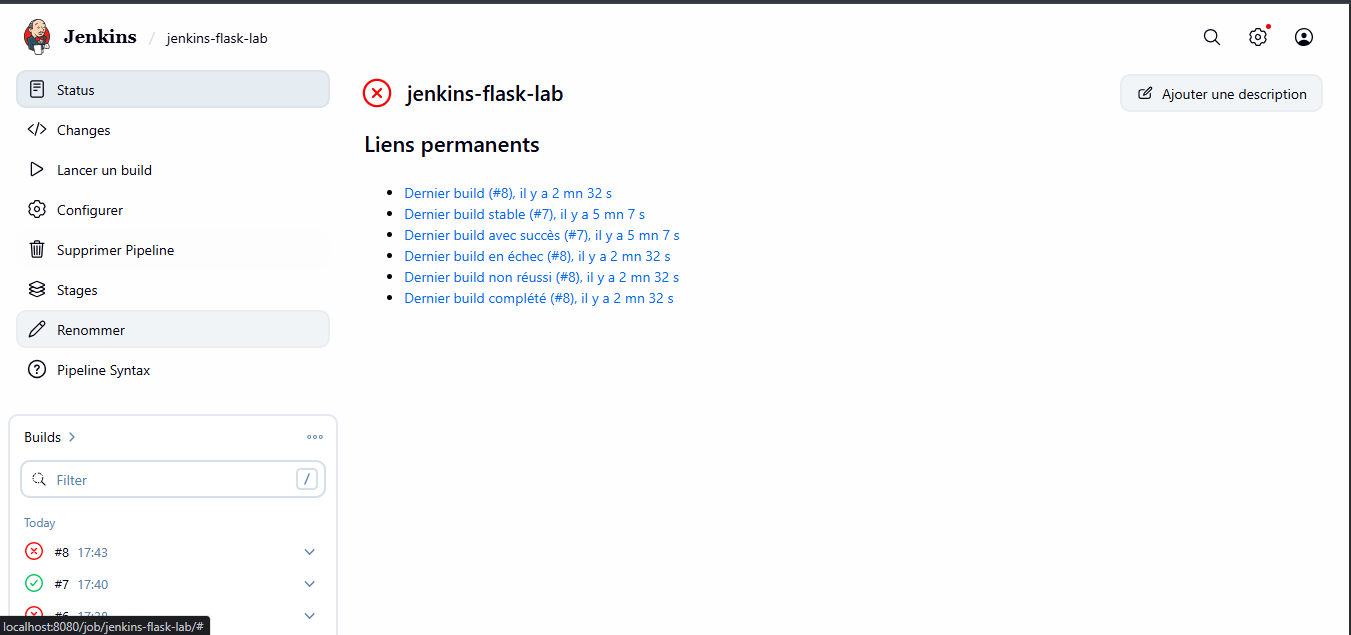
\includegraphics[width=0.92\textwidth]{img/build_failure.png}
\caption{Build 8 failing after the deliberate introduction of a failing test.}
\end{figure}

\begin{lstlisting}[caption={Console excerpt of build 8 (expected failure).}]
+ docker build -t jenkins-flask-lab:8 .
Successfully tagged jenkins-flask-lab:8
tests/test_app.py::test_home PASSED                                      [ 50%]
tests/test_app.py::test_health FAILED                                    [100%]

    def test_health():
        response = app.test_client().get("/health")
        assert response.status_code == 200
>       assert response.get_json() == {"status": "incorrect"}
E       AssertionError: assert {'status': 'ok'} == {'status': 'incorrect'}

Stage "Deploy" skipped due to earlier failure(s)
Stage "Verify" skipped due to earlier failure(s)
Pipeline failed. Check the stage that reported an error.
ERROR: script returned exit code 1
Finished: FAILURE
\end{lstlisting}

\subsection{Explanation}

The faulty version was not deployed because the pipeline is designed to stop as soon as a
stage fails: the following stages are not executed. The \texttt{jenkins-flask-app}
container therefore keeps serving the last valid version. This is exactly the expected
behaviour of a CI/CD pipeline: \emph{a version whose tests fail is never released}. The
correct assertion was then restored (commit \texttt{ed7a651}, ``Fix health test'') and a
new build was scheduled.

\section{Diagnostics and command outputs}

\subsection{Active containers}

\begin{lstlisting}
$ docker ps
NAMES               IMAGE                 STATUS          PORTS
jenkins-flask-app   jenkins-flask-lab:7   Up 14 minutes   0.0.0.0:8081->8000/tcp
jenkins             jenkins-docker-lab    Up 27 minutes   0.0.0.0:8080->8080/tcp, 0.0.0.0:50000->50000/tcp
\end{lstlisting}

\subsection{Docker client/server check from Jenkins}

\begin{lstlisting}
$ docker exec jenkins docker version --format "Client {{.Client.Version}} / Server {{.Server.Version}}"
Client 28.5.1 / Server 28.5.1
\end{lstlisting}

\subsection{Application images built by Jenkins}

\begin{lstlisting}
$ docker images jenkins-flask-lab
REPOSITORY           TAG   SIZE
jenkins-flask-lab    2     220MB
jenkins-flask-lab    3     220MB
jenkins-flask-lab    4     220MB
jenkins-flask-lab    5     220MB
jenkins-flask-lab    6     220MB
jenkins-flask-lab    7     220MB
jenkins-flask-lab    8     220MB
\end{lstlisting}

\subsection{Functional check from the Windows host}

\begin{lstlisting}
$ curl -s http://localhost:8081/health
{"status":"ok"}

$ curl -s http://localhost:8081/
<h1>Jenkins CI/CD Lab</h1><p>Version: 7</p>
\end{lstlisting}

\section{Part F: Blue-Green deployment and rollback (questions 19)}

\subsection{What is the difference between deployment and release?}
A \emph{deployment} is the technical operation that installs and starts a new version in
an environment (for example Green). A \emph{release} is the moment when that version is
actually exposed to users (traffic switch). A version can therefore be deployed without
being released: it runs in Green but no user is served by it before the switch. Deployment
is a technical decision, release is a product/business decision.

\subsection{Why is the new version deployed to Green before receiving production traffic?}
Because Green is identical to production but isolated from real traffic. The version can
be validated there (tests, health checks, monitoring) without any risk for users, who keep
using Blue. Any defect found then has no visible consequence.

\subsection{What component can route user requests to Blue or Green?}
A \emph{reverse proxy} or load balancer: \textbf{NGINX} (mentioned in the lab), but also
HAProxy, a cloud load balancer or DNS. The switch consists in changing the upstream and
reloading the proxy configuration.

\subsection{Why should Blue remain available after switching traffic to Green?}
To allow an immediate \emph{rollback}: if a problem appears on Green, traffic is sent
back to Blue, which still runs the stable version. Blue acts as a safety net during the
observation period.

\subsection{How can Jenkins automate the deployment, testing and approval steps?}
An extended pipeline can: build the image, deploy the Green container, run tests and
health checks on Green, wait for a manual approval (an \texttt{input} step or an approval
plugin), then update the NGINX configuration and reload it to switch traffic. Jenkins can
then run post-deployment monitoring and notify the team. On failure, the pipeline stops
and Blue keeps serving; everything is described in the Jenkinsfile, hence versioned and
reproducible.

\subsection{What is the main benefit of rollback in a Blue-Green deployment?}
It drastically reduces the recovery time (MTTR): going back to the stable version is almost
instantaneous (a simple proxy switch), with no rebuild or redeployment, and therefore
minimal impact on users.

\section{Part G: general questions (questions 20)}

\subsection{What is Jenkins, and what problem does it solve?}
Jenkins is an automation server that implements CI/CD workflows. It orchestrates source
retrieval, build, tests, analysis and deployment. It replaces manual, slow and
error-prone operations with automatic, traceable and reproducible pipelines, giving fast
feedback on every commit.

\subsection{What is the purpose of a Jenkinsfile?}
It is a text file that defines the pipeline ``as code'': environment, stages and commands.
Stored at the root of the repository, it is versioned with the code, can be changed
through Git, and Jenkins reads it on every build to execute the stages in order.

\subsection{What is the difference between Continuous Integration and Continuous Delivery?}
\emph{Continuous Integration} means integrating code frequently and automatically running
the build and tests on every commit to detect errors early. \emph{Continuous Delivery}
goes further: every version that passes the tests is automatically deployed to a
production-like environment and always remains ready to be released (promotion may require
manual approval). \emph{Continuous Deployment} releases automatically to production.

\subsection{What is the role of GitHub in this lab?}
GitHub hosts the source code and the Jenkinsfile. Jenkins is configured with ``Pipeline
script from SCM'' on the public repository URL and the \texttt{*/main} branch: it performs
a \texttt{fetch}/\texttt{checkout} on every build. A webhook could optionally trigger the
pipeline on each push, if Jenkins were reachable from GitHub.

\subsection{Why is Docker used in the pipeline?}
Docker packages the application and its dependencies into an immutable image. The
\textbf{same image} is used for tests and for deployment, which guarantees that the tested
environment is identical to the running one. Containers are lightweight, isolated and easy
to create or remove (test container with \texttt{--rm}, deployment container replaced on
every build).

\subsection{Why are automated tests executed before deployment?}
Tests automatically verify the expected behaviour (home page and \texttt{/health}
endpoint). If they fail, the pipeline stops: a faulty version is never deployed and the
running application is not replaced. This is the safety net of continuous delivery,
illustrated in Part E.

\subsection{What happens when a pipeline stage fails?}
The pipeline stops at the failing stage, the following stages are marked \emph{skipped},
the \texttt{post \{ failure \}} block runs and the build is
\textcolor{failred}{\textbf{FAILURE}}. In build 8, the failure of \texttt{test\_health}
prevented Deploy and Verify from running.

\subsection{What is the purpose of the Verify stage?}
It confirms that the deployment really succeeded, beyond the container merely starting:
HTTP requests with retries (\texttt{curl --fail --retry 10 --retry-delay 2}) check that
\texttt{/health} returns \texttt{\{"status":"ok"\}} and that the home page responds. It is
the end-to-end functional check.

\subsection{Why should credentials not be stored directly in a Jenkinsfile?}
The Jenkinsfile is versioned (often in a public repository) and visible to anyone with
access to the code: a password or token there would be exposed. The Jenkins credentials
store should be used instead (\texttt{credentials}, \texttt{withCredentials}) with an
identifier referenced from the Jenkinsfile.

\section{Conclusion}

The lab is complete: the GitHub repository contains the application, the tests, the
Dockerfile and the Jenkinsfile; Jenkins builds the image, runs the tests, deploys the
container and verifies the application; the deliberate test failure showed that the
pipeline correctly blocks the deployment and preserves the running version. The Windows
adaptations (containerized Jenkins with a Docker client, container name and
\texttt{host.docker.internal} for the checks) were necessary and are documented.

Possible improvements: a GitHub webhook to trigger builds automatically, a full Blue-Green
deployment with NGINX, a manual approval step in the pipeline, image security scanning and
post-deployment monitoring.

\appendix
\section{Main commands used}

\begin{lstlisting}
# Get the project
git clone https://github.com/Sadoune321/jenkins-flask-lab.git

# Build the Jenkins image (outside the application repository)
docker build -t jenkins-docker-lab C:\Users\tassili\Desktop\jenkins-docker

# Network and Jenkins container
docker network create jenkins-net
docker run -d --name jenkins --network jenkins-net -u root \
  -p 8080:8080 -p 50000:50000 \
  -v //var/run/docker.sock:/var/run/docker.sock \
  -v jenkins_home:/var/jenkins_home jenkins-docker-lab

# Check the Docker client inside Jenkins
docker exec jenkins docker version

# Check the application
curl http://localhost:8081/health
curl http://localhost:8081/
\end{lstlisting}

\end{document}
